%!TEX TS-program = xelatex
%!TEX options = -aux-directory=Debug -shell-escape -file-line-error -interaction=nonstopmode -halt-on-error -synctex=1 "%DOC%"
\documentclass{article}
\input{LaTeX-Submodule/template.tex}

% Additional packages & macros
\DeclareMathOperator{\sgn}{sgn}
\DeclareMathOperator{\sinc}{sinc}
\DeclareMathOperator{\erfc}{erfc}
\usepackage{makecell}

% Header and footer
\newcommand{\unitName}{Telecommunications and RF}
\newcommand{\unitTime}{Semester 2, 2023}
\newcommand{\unitCoordinator}{Dr Jacob Coetzee}
\newcommand{\documentAuthors}{Tarang Janawalkar}

\fancyhead[L]{\unitName}
\fancyhead[R]{\leftmark}
\fancyfoot[C]{\thepage}

% Copyright
\usepackage[
    type={CC},
    modifier={by-nc-sa},
    version={4.0},
    imagewidth={5em},
    hyphenation={raggedright}
]{doclicense}

\date{}

\begin{document}
%
\begin{titlepage}
    \vspace*{\fill}
    \begin{center}
        \LARGE{\textbf{\unitName}} \\[0.1in]
        \normalsize{\unitTime} \\[0.2in]
        \normalsize\textit{\unitCoordinator} \\[0.2in]
        \documentAuthors
    \end{center}
    \vspace*{\fill}
    \doclicenseThis
    \thispagestyle{empty}
\end{titlepage}
\newpage
%
\tableofcontents
\newpage
%
\section{Telecommunications Systems}
Telecommunication is the transmission of information over a distance
through some technology.

Telecommunications systems are designed to transmit information with as
little \textbf{deterioration} as possible while satisfying design
constraints, such as allowable transmittable energy and signal
bandwidth.

Signal deterioration commonly measures:
\begin{itemize}
    \item For Analog Systems: \textbf{Signal-to-Noise Ratio} (SNR) at
          the receiver output --- the ratio of the signal power to the
          noise power
    \item For Digital Systems: \textbf{Bit Error Rate} (BER) at the
          receiver output --- the ratio of the number of bits received
          in error to the total number of bits transmitted
\end{itemize}
\subsection{Analog and Digital Signals}
A system is either \textbf{analog} or \textbf{digital} based on the
possible amplitudes of waveforms it can handle.
\begin{itemize}
    \item \textbf{Analog Information Sources} produce values defined on
          a continuum:
          \begin{itemize}
              \item Human voice and other sounds
          \end{itemize}
    \item \textbf{Digital Information Sources} produce a finite set of
          possible symbols:
          \begin{itemize}
              \item Computer data
              \item MP3 encoder output
          \end{itemize}
\end{itemize}
\subsection{Communications System}
A communications system can be summarised by the following block
diagram:
\begin{figure}[H]
    \centering
    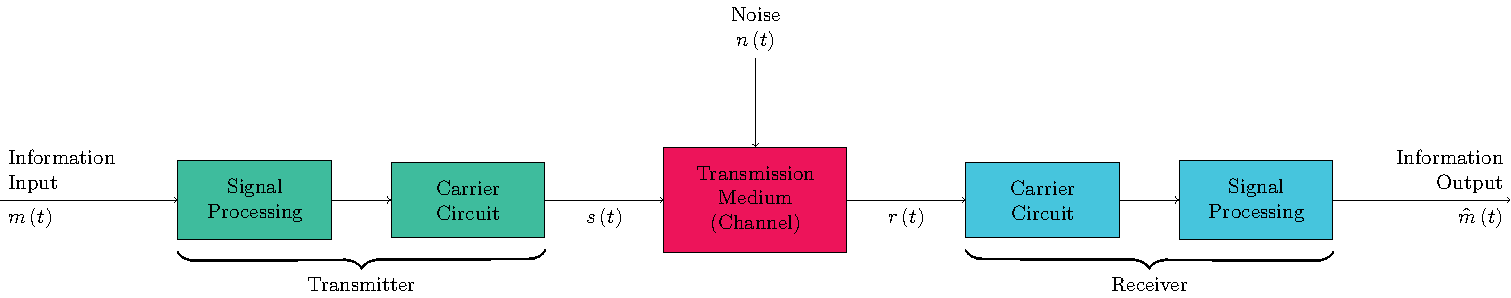
\includegraphics[width=\linewidth]{figures/communications_system.pdf}
    % \caption{} % \label{}
\end{figure}
where
\begin{itemize}
    \item \(m\left( t \right)\) is the information message signal
          (prior to conditioning for transmission)
    \item \(s\left( t \right)\) is the conditioned signal for transmission
    \item \(n\left( t \right)\) contains channel noise and interference
    \item \(r\left( t \right)\) is the received signal
    \item \(\hat{m}\left( t \right)\) is the reconstructed received
          message signal (where \(\hat{m}\left( t \right)\) usually
          approximates \(m\left( t \right)\))
\end{itemize}
\subsubsection{Transmitter}
The transmitter carries out \textbf{signal conditioning} by
transforming the signal to a more appropriate form before transmission
through the channel. Some examples of signal conditioning techniques
are prodived below.
\begin{itemize}
    \item \textbf{Low Pass Filtering} (LPF) restricts signal bandwidth
          to avoid wasting signal power on frequencies that are not
          transmitted by the channel and to avoid interference with other
          signals
    \item \textbf{Analog to Digital Conversion} (ADC) produces a
          digital word which represents a sample of the analog message
          waveform
    \item \textbf{Carrier Modulation} transfers the signal to a
          frequency band that is suitable for transmission through the
          channel
\end{itemize}
\subsubsection{Channel}
A communication channel refers to the physical medium that carries the
signal from the transmitter to the receiver. There are two types of
channels:
\begin{itemize}
    \item \textbf{Wired}: twisted pair copper telephone lines,
          waveguides, coaxial cables, fibre-optic cables
    \item \textbf{Wireless}: air, vacuums, sea water, optical fibres
\end{itemize}
General principles of communications always apply regardless of the type
of channel. However, certain conditioning methods are better suited to
certain channels.

Channels often \textbf{attenuate} signals (reduce their amplitude or
strength) through
\begin{itemize}
    \item random noise
    \item interference from other sources
\end{itemize}
and therefore it is a key consideration in the design of a communications system.
\subsubsection{Receiver}
The receiver acts as the inverse of a transmitter. The receiver:
\begin{enumerate}
    \item \textbf{Demodulates} the received signal by stripping the
          carrier from the received signal \(r\left( t \right)\).
    \item \textbf{Filters} out noise and interference from the
          demodulated signal.
    \item \textbf{Reconstructs} an estimate of the original message
          signal \(\hat{m}\left( t \right)\).
\end{enumerate}
Due to the finite nature of the SNR, the estimated output of an analog
signal can never be exactly equal to the original signal\footnote{A
    perfect reconstruction requires an infinite SNR which is impractical.}.
However, it is often possible to reconstruct a digital signal exactly
using error detection and correction techniques at the receiver.
\subsubsection{Information Sources}
As discussed before, an information source can be classified as either
\textbf{analog} or \textbf{digital}. Analog signals can be modulated or
transmitted directly, or converted to digital data and transmitted
using digital modulation techniques.

An analogue signal to be transmitted is called the \textbf{message
signal} and is denoted \(m\left( t \right)\). The spectral components
of this signal lie within a finite bandwidth \(W\), such that \(M\left(
f \right) = 0\) for \(\abs*{f} > W\), where \(M\left( f \right)\) is
the Fourier Transform of \(m\left( t \right)\). This signal's bandwidth
is limited to prevent interference with other signals.

Many kinds of message signals can be considered:
\begin{itemize}
    \item Audio
    \item Video
    \item Computer data
    \item Telemetry (measurements)
    \item Soundings (RADAR, SONAR)
    \item A mixure of the above (i.e., data over voice)
\end{itemize}
\subsection{Modulation}
The process of modulation produces a signal that is suitable for
transmission through the channel by transforming the message signal
\(m\left( t \right)\) to a new signal \(s\left( t \right)\).

Modulation is often performed with respect to another signal, called
the \textbf{carrier} signal \(c\left( t \right)\). Here the message
\textit{modulates} the carrier to produce the transmitted signal
\(s\left( t \right)\).
\subsubsection{Benefits of Modulation}
\begin{itemize}
    \item Modulation shifts the spectral content of a message onto a
          suitable band. As the size of an antenna is related to the
          wavelength of a signal, higher carrier frequencies require
          smaller antennas.
    \item Modulation facilitates multiplexing, where multiple signals
          are transmitted over the same spectrum. This is because the
          frequency spectrum can be divided into non-overlapping
          frequency bands, each of which can carry a separate signal.
    \item Modulation provides some control over noise and interference
          by choosing a bandwidth that is smaller than the allocated
          channel bandwidth.
\end{itemize}
\subsubsection{Convolution and Modulation}
Consider two time domain signals \(m\left( t \right)\) and \(c\left( t
\right)\) and their Fourier Transforms \(M\left( f \right)\) and
\(C\left( f \right)\) respectively.

The \textbf{Convolution Property} demonstrates:
\begin{align*}
    m\left( t \right) \ast c\left( t \right) & = y\left( t \right) &  & \text{Convolution in Time Domain}         \\
    M\left( f \right) C\left( f \right)      & = Y\left( f \right) &  & \text{Multiplication in Frequency Domain}
\end{align*}
The \textbf{Modulation property} demonstrates:
\begin{align*}
    m\left( t \right) c\left( t \right)      & = y\left( t \right) &  & \text{Multiplication in Time Domain}   \\
    M\left( f \right) \ast C\left( f \right) & = Y\left( f \right) &  & \text{Convolution in Frequency Domain}
\end{align*}
\subsubsection{Carrier Signal}
The carrier signal \(c\left( t \right)\) is a sinusoidal signal of the
form:
\begin{equation*}
    c\left( t \right) = A_c \cos{\left( 2 \pi f_c t + \phi \right)}
\end{equation*}
where \(A_c\) is the amplitude, \(f_c\) is the frequency and \(\phi\) is
the phase of the carrier signal.
\subsubsection{Signal Properties}
The \textbf{energy} of a signal \(x\left( t \right)\) is defined as:
\begin{equation*}
    E_x = \int_{-\infty}^{\infty} \abs*{x\left( t \right)}^2 \odif{t}
\end{equation*}
The rate at which energy is transmitted is called the \textbf{power} of
the signal, and is defined as:
\begin{equation*}
    P_x = \lim_{T \to \infty} \frac{1}{T} \int_{-T/2}^{T/2} \abs*{x\left( t \right)}^2 \odif{t}
\end{equation*}
where \(T\) is the time period over which the power is measured.
\subsection{Amplitude Modulation Schemes}
A message signal \(m\left( t \right)\) with bandwidth \(W\) can be
amplitude modulated by mixing (multiplying) the signal with a carrier
signal \(c\left( t \right)\):
\begin{equation*}
    c\left( t \right) = A_c \cos{\left( 2 \pi f_c t \right)}
\end{equation*}
with amplitude \(A_c\) and carrier frequency \(f_c \gg W\).

This section will consider:
\begin{itemize}
    \item Double Side Band --- Suppressed Carrier (DSB-SC) modulation
    \item Double Side Band --- Full Carrier (DSB-FC) modulation, or
          simply conventional Amplitude Modulation (AM)
    \item Single Side Band (SSB) modulation
\end{itemize}
\subsubsection{Double Side Band --- Suppressed Carrier (DSB-SC)}
The transmitted signal is defined as:
\begin{equation*}
    s\left( t \right) = m\left( t \right) c\left( t \right) = A_c m\left( t \right) \cos{\left( 2 \pi f_c t \right)}.
\end{equation*}
In the frequency domain, the message signal is shifted to the carrier
frequency at \(\pm f_c\) and the magnitude is halved.
\begin{equation*}
    S\left( f \right) = \frac{1}{2} A_c \left[ M\left( f - f_c \right) + M\left( f + f_c \right) \right]
\end{equation*}
Assuming no channel noise, the received signal can be represented as:
\begin{equation*}
    r\left( t \right) = s\left( t \right) = A_c m\left( t \right) \cos{\left( 2 \pi f_c t \right)}
\end{equation*}
This signal can be demodulated coherently by multiplying a sinusoidal
signal of the same frequency as the carrier. Suppose we generate the
sinusoidal signal \(\cos{\left( 2 \pi f_c t + \phi \right)}\) where
\(\phi\) is the phase of the sinusoid.
\begin{align*}
    y\left( t \right) & = r\left( t \right) \cos{\left( 2 \pi f_c t + \phi \right)}                                                                                                                                             \\
                      & = A_c m\left( t \right) \cos{\left( 2 \pi f_c t \right)} \cos{\left( 2 \pi f_c t + \phi \right)}                                                                                                        \\
                      & = \frac{1}{2} A_c m\left( t \right) \left[ \cos{\left( 4 \pi f_c t + \phi \right)} + \cos{\left( -\phi \right)} \right]                                                                                 \\
                      & = \underbrace{\frac{1}{2} A_c m\left( t \right) \cos{\left( \phi \right)}}_{\text{filter out}} + \underbrace{\frac{1}{2} A_c m\left( t \right) \cos{\left( 4 \pi f_c t + \phi \right)}}_{\text{reject}}
\end{align*}
As the frequency content of the message signal \(m\left( t \right)\) is
limited to \(W\), a lowpass filter can be used to remove the high
frequency component centred at \(2f_c\). The output of this filter is
then
\begin{equation*}
    \hat{m}\left( t \right) = \frac{1}{2} A_c m\left( t \right) \cos{\left( \phi \right)}.
\end{equation*}
Note that \(m\left( t \right)\) is multiplied by \(\cos{\left( \phi
    \right)}\), meaning the power of the message signal is reduced by a
factor of \(\cos^2{\left( \phi \right)}\). It is therefore important to
choose \(\phi\) such that \(\cos{\left( \phi \right)}\) is as close to
\(1\) as possible. This demonstrates a need for a phase-coherent or
synchronous demodulator, i.e., the phase of the locally generated
sinusoid should be identical to the received carrier signal.
\subsubsection{Double Side Band --- Full Carrier (DSB-FC)}
This scheme is similar to DSB-SC, however the carrier is sent along
with the modulated signal. We begin by defining an envelope signal
\(g\left( t \right)\) by amplifying and biasing the message signal, so
that:
\begin{equation*}
    g\left( t \right) = 1 + \mu m_n\left( t \right)
\end{equation*}
where the \textbf{modulation index} \(0 < \mu \leqslant 1\) is chosen to
ensure \(g\left( t \right) > 0\).
\(m_n\left( t \right)\) is the normalised message signal defined as
\begin{equation*}
    m_n\left( t \right) = \frac{m\left( t \right)}{\max{\abs*{m\left( t \right)}}}
\end{equation*}
such that \(\abs*{m_n\left( t \right)} \leqslant 1\).
The transmitted signal is then defined as:
\begin{equation*}
    s\left( t \right) = g\left( t \right) c\left( t \right) = A_c \left[ 1 + \mu m_n\left( t \right) \right] \cos{\left( 2 \pi f_c t \right)}.
\end{equation*}
In the frequency domain, we observe similar behaviour, with impulses at
\(\pm f_c\).
\begin{equation*}
    S\left( f \right) = \frac{1}{2} A_c \mu \left[ M\left( f - f_c \right) + M\left( f + f_c \right) \right] + \frac{1}{2} A_c \left[ \delta\left( f - f_c \right) + \delta\left( f + f_c \right) \right]
\end{equation*}
The modulation index can be determined from the AM signal using the
following equation:
\begin{equation*}
    \mu = \frac{A_{\mathrm{max}} - A_{\mathrm{min}}}{A_{\mathrm{max}} + A_{\mathrm{min}}} = \frac{\max{\abs*{m\left( t \right)}}}{\max{\abs*{c\left( t \right)}}} % chktex 35
\end{equation*}
where \(A_{\mathrm{max}}\) and \(A_{\mathrm{min}}\) are the maximum and % chktex 35
minimum amplitudes of the envelope signal \(g\left( t \right)\). This
value is chosen to be as close to \(1\) as possible to maximise the
power of the transmitted signal. Increasing \(\mu\) beyond 1
overmodulates the signal, resulting in a full-wave rectified version of
the signal.

Modulation efficiency is the percentage of the total power of the
modulated signal that conveys information
\begin{equation*}
    \eta = \frac{\text{sideband power}}{\text{total power}} \times 100\%
\end{equation*}
As the total power comprises of both the sideband power and carrier
power, the DSB-FC scheme is very inefficient. This is because the
carrier signal does not contain any useful information, and therefore
the power of the carrier is wasted. This can be seen when transmitting a
sinusoidal message signal,
\begin{itemize}
    \item Carrier power: \(\frac{1}{2} A_c^2\)
    \item Sideband power: \(\frac{1}{4} A_c^2 \mu^2\)
    \item Total power: \(\frac{1}{2} A_c^2 \left( 1 + \frac{1}{2}\mu^2
          \right)\)
    \item Modulation efficiency: \(\frac{\frac{1}{4} A_c^2
          \mu^2}{\frac{1}{2} A_c^2 \left( 1 + \frac{1}{2}\mu^2 \right)}
          = \frac{\mu^2}{2 + \mu^2}\)
\end{itemize}
The maximum efficiency is achieved when \(\mu = 1\), i.e., which is \(33\%\).
This scheme is often used in AM medium-wave (MW) systems.

To demodulate a DSB-FC signal, we can use an envelope detector. In this
circuit, we need to calculate the minimum and maximum frequency that
the tuned circuit can respond to:
\begin{equation*}
    f_0 = \frac{1}{2 \pi \sqrt{LC_1}}
\end{equation*}
and calculate the break frequency of the lowpass filter:
\begin{equation*}
    f_b = \frac{1}{2 \pi R C_2}
\end{equation*}
\subsubsection{Single Side Band (SSB)}
As the double side band schemes produce a signal with twice the
bandwidth of the message signal, consider either the lower or upper
sidebands of the modulated signal. We can attempt to use a filter to
remove the unwanted sideband, however there are two issues with this
approach:
\begin{enumerate}
    \item The filter is particularly difficult to implement when
          \(m\left( t \right)\) has a large concentration of power
          close to \(f = 0\)
    \item The filter must have a very sharp cutoff in the vicinity of
          the carrier frequency
\end{enumerate}
Instead, we can use a phase shift method through the use of a Hilbert
transform. The Hilbert transform of a signal \(m\left( t \right)\) is
defined as
\begin{equation*}
    \hat{m}\left( t \right) = m\left( t \right) \ast \frac{1}{\pi t}
\end{equation*}
The result of this operation is more easily understood in the frequency domain.
\begin{equation*}
    \hat{M}\left( f \right) = -j \sgn{\left( f \right)} M\left( f \right) =
    \begin{cases}
        -j M\left( f \right) & f > 0 \\
        j M\left( f \right)  & f < 0
    \end{cases}
\end{equation*}
so that negative frequency components of \(m\) are phase shifted by \(+90^{\circ}\) (\(+\pi/2\)) and
positive frequency components are phase shifted by \(-90^{\circ}\) (\(-\pi/2\)).
The magnitude remains unchanged.

Using this transform, we can define SSB signals as:
\begin{gather*}
    s_{\mathrm{USB}}\left( t \right) = A_c \left[ m\left( t \right) \cos{\left( 2 \pi f_c t \right)} - \hat{m}\left( t \right) \sin{\left( 2 \pi f_c t \right)} \right] \\
    s_{\mathrm{LSB}}\left( t \right) = A_c \left[ m\left( t \right) \cos{\left( 2 \pi f_c t \right)} + \hat{m}\left( t \right) \sin{\left( 2 \pi f_c t \right)} \right]
\end{gather*}
or compactly,
\begin{equation*}
    s\left( t \right) = m\left( t \right) c\left( t \right) \pm \hat{m}\left( t \right) \hat{c}\left( t \right)
\end{equation*}
These signals can be demodulated coherently using the same process as
the DSB-SC scheme. Again assuming that there is no channel noise,
\begin{equation*}
    r\left( t \right) = s\left( t \right) = A_c m\left( t \right) \cos{\left( 2\pi f_c t \right)} \pm A_c \hat{m}\left( t \right) \sin{\left( 2\pi f_c t \right)}
\end{equation*}
\begin{align*}
    y\left( t \right) & = r\left( t \right) \cos{\left( 2 \pi f_c t + \phi \right)}                                                                                                                                                                                                                                                                                                     \\
                      & = \left[ A_c m\left( t \right) \cos{\left( 2\pi f_c t \right)} \pm A_c \hat{m}\left( t \right) \sin{\left( 2\pi f_c t \right)} \right] \cos{\left( 2 \pi f_c t + \phi \right)}                                                                                                                                                                                  \\
                      & = A_c m\left( t \right) \cos{\left( 2\pi f_c t \right)} \cos{\left( 2 \pi f_c t + \phi \right)} \pm A_c \hat{m}\left( t \right) \sin{\left( 2\pi f_c t \right)} \cos{\left( 2 \pi f_c t + \phi \right)}                                                                                                                                                         \\
                      & = \frac{1}{2} A_c m\left( t \right) \left[ \cos{\left( \phi \right)} + \cos{\left( 4 \pi f_c t + \phi \right)} \right] \pm \frac{1}{2} A_c \hat{m}\left( t \right) \left[ -\sin{\left( \phi \right)} + \sin{\left( 4 \pi f_c t + \phi \right)} \right]                                                                                                          \\
                      & = \underbrace{\frac{1}{2} A_c \left[ m\left( t \right) \cos{\left( \phi \right)} \mp \hat{m}\left( t \right) \sin{\left( \phi \right)} \right]}_{\text{filter out}} + \underbrace{\frac{1}{2} A_c \left[ m\left( t \right) \cos{\left( 4 \pi f_c t + \phi \right)} \pm \hat{m}\left( t \right) \sin{\left( 4 \pi f_c t + \phi \right)} \right]}_{\text{reject}}
\end{align*}
This gives the output
\begin{equation*}
    \hat{m}\left( t \right) = \frac{1}{2} A_c \left[ m\left( t \right) \cos{\left( \phi \right)} \mp \hat{m}\left( t \right) \sin{\left( \phi \right)} \right]
\end{equation*}
Note the \(\hat{m}\left( t \right)\) term on the right hand side of the
equation is referring to the Hilbert transform of \(m\left( t \right)\),
not the output of the demodulator.
\section{Angle Modulation}
AM suffers from poor noise performance, as amplitude variations in the
received signal cannot be removed from the demodulated signal. Angle
modulation schemes overcome this issue by modulating the phase or
frequency of the carrier signal.
\subsection{Carrier Signal}
In these schemes, the message signal is modulated onto the angle
\(\theta\left( t \right)\) of the carrier signal:
\begin{gather*}
    s\left( t \right) = A_c \cos{\left( \theta\left( t \right) \right)} \\
    \theta\left( t \right) = 2\pi f_c t + \phi\left( t \right)
\end{gather*}
In \textbf{phase modulation} (PM), variations in the message signal are
encoded into the phase:
\begin{equation*}
    \phi\left( t \right) = k_p m\left( t \right)
\end{equation*}
where \(k_p\) is the \textbf{phase deviation} constant.

\textbf{Frequency modulation} (FM) considers the frequency deviation
from the modulation frequency \(f_c\):
\begin{equation*}
    f_i - f_c = k_f m\left( t \right)
\end{equation*}
where \(f_i\) is the instantaneous frequency of the carrier signal and
\(k_f\) is the \textbf{frequency deviation} constant. To determine the
phase \(\phi\), consider the time derivative of the angle
\(\theta\left( t \right)\) with arbitrary frequency \(f\)
\begin{align*}
    \odv{\theta\left( t \right)}{t} & = \odv*{\left( 2\pi f t + \phi \right)}{t}                        \\
    \odv{\theta\left( t \right)}{t} & = 2\pi f_i                                                        \\
    \theta\left( t \right)          & = 2\pi \int_0^t f_i \odif{\tau}                                   \\
    \theta\left( t \right)          & = 2\pi \int_0^t f_c + k_f m\left( \tau \right) \odif{\tau}        \\
    \theta\left( t \right)          & = 2\pi f_c t + 2\pi k_f \int_0^t m\left( \tau \right) \odif{\tau}
\end{align*}
\subsubsection{Phase Modulation}
A phase modulated signal is defined as:
\begin{equation*}
    s\left( t \right) = A_c \cos{\left( 2\pi f_c t + k_p m\left( t \right) \right)}
\end{equation*}
with
\begin{equation*}
    \theta\left( t \right) = 2\pi f_c t + k_p m\left( t \right)
\end{equation*}
where \(k_p\) is the \textbf{phase deviation} constant.
\subsubsection{Frequency Modulation}
A frequency modulated signal is defined as:
\begin{equation*}
    s\left( t \right) = A_c \cos{\left( 2\pi f_c t + 2\pi k_f \int_0^t m\left( \tau \right) \odif{\tau} \right)}
\end{equation*}
with
\begin{equation*}
    \theta\left( t \right) = 2\pi f_c t + 2\pi k_f \int_0^t m\left( \tau \right) \odif{\tau}
\end{equation*}
where \(k_f\) is the \textbf{frequency deviation} constant.
\subsubsection{Instantaneous Frequency}
The instantaneous frequency \(f_i\) may be determined from these
signals by considering the time derivative of \(\theta\).

In PM,
\begin{align*}
    \odv{\theta}{t} & = 2\pi f_c + k_p \odv*{m\left( t \right)}{t}                                                                                               \\
                    & = 2\pi \left( f_c + \frac{k_p}{2\pi} \odv*{m\left( t \right)}{t} \right) \implies f_i = f_c + \frac{k_p}{2\pi} \odv*{m\left( t \right)}{t}
\end{align*}
In FM,
\begin{align*}
    \odv{\theta}{t} & = 2\pi f_c + 2\pi k_f m\left( t \right)                                                      \\
                    & = 2\pi \left( f_c + k_f m\left( t \right) \right) \implies f_i = f_c + k_f m\left( t \right)
\end{align*}
\subsubsection{Modulation Index}
The modulation index \(\beta\) is defined as the ratio of the maximum
frequency deviation to the modulating frequency of the message signal.
In PM, if we rewrite the phase \(\phi\left( t \right)\) as,
\begin{align*}
    \phi\left( t \right) & = k_p \max{\abs*{m\left( t \right)}} \frac{m\left( t \right)}{\max{\abs*{m\left( t \right)}}} \\
                         & = \beta_p m_n\left( t \right)
\end{align*}
then \(\beta_p\) is the modulation index for PM.
By definition, FM has a modulation index of \(\beta_f = \frac{k_f \max{\abs*{m\left( t \right)}}}{B}\)
where \(B\) is the bandwidth of the message signal.
\subsubsection{Maximum Phase and Frequency Deviation}
The maximum phase deviation \(\Delta p\) and maximum frequency
deviation \(\Delta f\) are defined as:
\begin{equation*}
    \Delta p = k_p \max{\abs*{m\left( t \right)}} \qquad \Delta f = k_f \max{\abs*{m\left( t \right)}}
\end{equation*}
\subsubsection{Carson's Rule}
Phase and frequency modulation generally expand the bandwidth of a
signal. The modulated signals bandwidth \(W\) may be approximated by
Carson's rule:
\begin{equation*}
    W = 2B \left( \beta + 1 \right)
\end{equation*}
\subsubsection{Summary of Angle Modulation Definitions}
% \begin{noindent}
\begin{table}[H]
    \centering
    \begin{tabular}{lcc}
        \toprule
                                                                                  & \textbf{Phase Modulation}                                                     & \textbf{Frequency Modulation}                                                                              \\
        \midrule
        \makecell[l]{\textbf{Modulated} \\ \textbf{Signal} \(s\left( t \right)\)} & \(\displaystyle A_c \cos{\left( 2\pi f_c t + k_p m\left( t \right) \right)}\) & \(\displaystyle A_c \cos{\left( 2\pi f_c t + 2\pi k_f \int_0^t m\left( \tau \right) \odif{\tau} \right)}\) \\[1em]
        \textbf{Phase} \(\phi\left( t \right)\)                                   & \(\displaystyle k_p m\left( t \right)\)                                       & \(\displaystyle 2\pi k_f \int_0^t m\left( \tau \right) \odif{\tau}\)                                       \\[1em]
        \makecell[l]{\textbf{Instantaneous} \\ \textbf{Frequency} \(f_i\)}        & \(\displaystyle f_c + \frac{k_p}{2\pi} \odv*{m\left( t \right)}{t}\)          & \(\displaystyle f_c + k_f m\left( t \right)\)                                                              \\[1em]
        \makecell[l]{\textbf{Modulation} \\ \textbf{Index}}                       & \(\displaystyle \beta_p = k_p \max{\abs*{m\left( t \right)}}\)                & \(\displaystyle \beta_f = \frac{k_f \max{\abs*{m\left( t \right)}}}{B}\)                                   \\[1em]
        \makecell[l]{\textbf{Maximum} \\ \textbf{Deviation}}                      & \(\displaystyle \Delta p = k_p \max{\abs*{m\left( t \right)}}\)               & \(\displaystyle \Delta f = k_f \max{\abs*{m\left( t \right)}}\)                                            \\[1em]
        \bottomrule
    \end{tabular}
    % \caption{} % \label{}
\end{table}
% \end{noindent}
\subsection{Narrowband Angle Modulation}
When \(\beta \ll 1\), angle modulation is referred to as narrowband
angle modulation. The modulated signal can be approximated as:
\begin{align*}
    s\left( t \right) & = A_c \cos{\left( 2 \pi f_c t + \phi\left( t \right) \right)}                                                                                                     \\
                      & = A_c \cos{\left( 2 \pi f_c t \right)} \cos{\left( \phi\left( t \right) \right)} - A_c \sin{\left( 2 \pi f_c t \right)} \sin{\left( \phi\left( t \right) \right)} \\
                      & = A_c \cos{\left( 2 \pi f_c t \right)} - A_c \phi\left( t \right) \sin{\left( 2 \pi f_c t \right)}
\end{align*}
This is equivalent to a DSB-FC signal with a phase modulated carrier, as
the message signal is now modulated onto a sine carrier instead of
cosine. The modulated signal bandwidth \(W\) is approximately \(2B\).

Narrowband angle modulation (low-index angle modulation) does not
provide better noise immunity than AM, and is seldom used on its own in
practical communication systems.
\subsection{Wideband Angle Modulation}
Assuming the message signal is a sinusoidal signal, \(\phi\left( t
\right) = \beta \sin{\left( 2 \pi f_m t \right)}\),
\begin{align*}
    s\left( t \right) & = A_c \cos{\left( 2 \pi f_c t + \beta \sin{\left( 2 \pi f_m t \right)} \right)}                                                                                                                       \\
                      & = A_c \cos{\left( 2 \pi f_c t \right)} \cos{\left( \beta \sin{\left( 2 \pi f_m t \right)} \right)} - A_c \sin{\left( 2 \pi f_c t \right)} \sin{\left( \beta \sin{\left( 2 \pi f_m t \right)} \right)}
\end{align*}
To simplify this expression, we can use Bessel functions. Notably
\begin{align*}
    \cos{\left( \beta \sin{\left( 2 \pi f_m t \right)} \right)} & = J_0\left( \beta \right) + 2 \sum_{n=1}^{\infty} J_{2n}\left( \beta \right) \cos{\left( 2 \pi \left( 2n \right) f_m t \right)} \\
    \sin{\left( \beta \sin{\left( 2 \pi f_m t \right)} \right)} & = 2 \sum_{n=1}^{\infty} J_{2n-1}\left( \beta \right) \sin{\left( 2 \pi \left( 2n-1 \right) f_m t \right)}
\end{align*}
where \(J_n\left( \beta \right)\) are Bessel functions of the first kind
and order \(n\), evaluated at \(\beta\).

These results can be used to show that a wideband FM modulated signal
can be expressed as:
\begin{equation*}
    s\left( t \right) = \sum_{n = -\infty}^\infty A_c J_n\left( \beta \right) \cos{\left( 2 \pi \left( f_c + n f_m \right) t \right)}
\end{equation*}
so that the carrier frequency is located at \(2 \pi f_c\) with magnitude \(A_c J_0\left( \beta \right)\), with an
infinite number of sidebands at \(2 \pi \left( f_c \pm n fm \right)\) with magnitudes \(A_c J_{\pm n}\left( \beta \right)\).

When deciding the number of sidebands \(n\) to include, consider
\begin{equation*}
    \abs*{J_{\pm n}\left( \beta \right)} \geqslant 0.1
\end{equation*}
For large values of \(\beta\), \(n \approx \beta\) is sufficient.

According to Carson's rule, \(W = 2 f_m \left( \beta + 1 \right)\)
contains at least \(98\%\) of the signal power.
\subsubsection{Bessel Function Properties}
The Bessel functions of the first kind \(J_n\left( x \right)\) are
defined as the solutions to the Bessel differential equation
\begin{equation*}
    x^2 \odv[order=2]{y}{x} + x \odv{y}{x} + \left( x^2 - n^2 \right) y = 0
\end{equation*}
\begin{itemize}
    \item \(J_n\left( \beta \right)\) is a real function
    \item \(J_n\left( \beta \right) = J_{-n}\left( \beta \right)\)
    \item \(\sum_{n = -\infty}^\infty J_n^2\left( \beta \right) = 1\)
\end{itemize}
For small values of \(\beta\),
\begin{itemize}
    \item \(J_0\left( \beta \right) = 1\)
    \item \(J_1\left( \beta \right) = \beta/2\)
    \item \(J_n\left( \beta \right) = 0\) for \(n > 2\)
\end{itemize}
\subsection{Effect of Bandwidth}
Rewriting Carson's rule using \(\beta\),
\begin{equation*}
    W = 2B \left( \beta + 1 \right) =
    \begin{cases}
        2B \left( k_p \max{\abs*{m\left( t \right)}} + 1 \right) & \text{PM} \\
        2 \left( k_f \max{\abs*{m\left( t \right)}} + B \right)  & \text{FM}
    \end{cases}
\end{equation*}
From these equations
\begin{itemize}
    \item Increasing the amplitude of the modulating signal has the
          same effect in both PM and FM.
    \item Increase the message signal bandwidth \(B\) has a greater
          effect on the bandwidth of a PM signal than for FM.
\end{itemize}
\subsection{Angle Modulator Implementation}
FM can be generated using a Voltage Controlled Oscillator (VCO). A
varactor diode is a capacitor whose capacitance changes with applied
voltage. This capacitor can be used in the tuned circuit of an
oscillator. If the message signal is applied to the varactor, the
output frequency of the oscillator will change in accordance with the
message signal.

The time varying capacitance of the varactor diode is given by
\begin{equation*}
    C_v\left( t \right) = C_a + k_0 m\left( t \right)
\end{equation*}
\begin{itemize}
    \item When \(m\left( t \right) = 0\), the frequency of the tuned
          circuit is given by
          \begin{equation*}
              f_i = f_c = \frac{1}{2 \pi \sqrt{L C_a}}
          \end{equation*}
    \item When \(m\left( t \right) \neq 0\), the frequency of the tuned
          circuit is given by
          \begin{equation*}
              f_i = \frac{1}{2 \pi \sqrt{L \left( C_a + k_0 m\left( t \right) \right)}} = \frac{1}{2 \pi \sqrt{L C_a \left( 1 + k_0 m\left( t \right) / C_a \right)}} = f_c \frac{1}{\sqrt{1 + k_0 m\left( t \right) / C_a}}
          \end{equation*}
\end{itemize}
Narrowband FM can be converted to wideband using a
narrowband-to-wideband convertor by multiplying the frequencies of the
narrowhand signal.
\subsection{Demodulating Angle Modulated Signals}
FM demodulators are implemented by generating an AM signal whose
amplitude is proportional to the instantaneous frequency of the FM
signal. We can then use an AM demodulator to recover the message
signal.

In such a circuit, the LTI system is a differentiator whose frequency
response is approximately a straight line in the frequency band of the
FM signal. \(\abs*{H} = 2 \pi f\).
\subsection{AM vs. FM}
\begin{itemize}
    \item FM capture effect: When two FM signals are received, the
          stronger signal is demodulated and the weaker signal is
          ignored.
          \begin{itemize}
              \item The complete suppression of the weaker signal
                    occurs at the receiver limited, where it is treated
                    as noise and rejected.
              \item When both signals are of equal strength, the
                    receiver may switch between the two signals.
          \end{itemize}
    \item FM requires a higher bandwidth \(W_{\mathrm{AM}} <
          W_{\mathrm{FM}}\).
    \item FM rejects amplitude noise cause by lightning and other
          man-made noise.
    \item AM demodulators: envelope detector, product detector.
    \item FM demodulators: PLL, ratio detector, frequency
          discriminator, slope detector.
\end{itemize}
\section{Digital Baseband Modulation}
A source encoder converts an analog signal into a sequence of binary
digits (bits). Digital modulation is used to transmit digital
information over an additive white Gaussian noise (AWGN) channel.
\begin{definition}[Baseband Channel]
    A baseband channel is a channel that includes the zero frequency
    \(f = 0\), and there is no need to transmit a carrier signal.
\end{definition}
\begin{definition}[Bandpass Channel]
    A communication channel that is far from the zero frequency is
    known as a bandpass channel, and such a signal is impressed on a
    sinusoidal carrier, that shifts the signal to the desired frequency
    band that is \textit{passed} by the channel.
\end{definition}
Pulse code modulation (PCM) is a method used to digitally represent a
sampled analog signal. To transmit these digits, we can use electrical
pulses to represent binary digits.
\begin{definition}[Bit]
    A bit is a binary digit, i.e., a digit that can take on one of two
    values; 0 or 1.
\end{definition}
\begin{definition}[Digital Symbol]
    A digital symbol refers to a sequence of several bits.
    For a sequence of \(k\) bits, there are \(M = 2^k\) unique symbols.
\end{definition}
\subsection{Waveform Representation of Digital Signals}
\textbf{Symbol rate} \(R_s\) is the number of symbols transmitted
per second, measured in \unit{symbols/s}.

\textbf{Bit rate} \(R_b\) is the number of bits transmitted
per second, measured in \unit{bits/s}.

Symbol rate and bit rate are related by
\begin{equation*}
    R_b = k R_s
\end{equation*}
where \(k\) is the number of bits per symbol. When a symbol contains
only one bit (\(k = 1\)), \(R_b = R_s\).

The duration of a single bit, or symbol can be determined using the
reciprocal of each quantity:
\begin{equation*}
    T_s = \frac{1}{R_s} \qquad T_b = \frac{1}{R_b}
\end{equation*}
These quantities are related by
\begin{equation*}
    T_b = \frac{1}{k} T_s
\end{equation*}
To effectively transmit digital signals through an analog channel, each
pulse must carry sufficient energy either by increasing the amplitude
or duration of each pulse.
\subsubsection{Antipodal and Orthogonal Signalling}
Antipodal signalling is a method of transmitting digital signals where
the information bit 1 is represented by a pulse \(p\left( t \right)\)
of duration \(T_b\), and the information bit 0 is represented by
\(-p\left( t \right)\).

In orthogonal signalling, information is represented by two orthogonal
pulses \(p_1\left( t \right)\) and \(p_2\left( t \right)\) such that
\begin{equation*}
    \int_{0}^{T_b} p_1\left( t \right) p_2\left( t \right) \odif{t} = 0
\end{equation*}
Each of the above methods require precise synchronisation between the
receiver and transmitter.
\subsubsection{Not-Return To Zero}
A non-return to zero (NRZ) \textbf{line code} is a binary code in which
bits are represented by two different levels of voltage.

For bipolar NRZ, the bit 1 is represented by a positive voltage, and
the bit 0 is represented by a negative voltage.

For unipolar NRZ, the bit 1 is represented by a positive voltage, and
the bit 0 is represented by a zero voltage.
\subsubsection{Pulse Amplitude Modulation}
In pulse amplitude modulation (PAM), the amplitude of a pulse is varied
between various voltage levels to represent digital symbols of \(k\)
bits. The number of voltage levels is given by \(M = 2^k\).
\subsection{Signal Bandwidth}
The bandwidth of a signal provides a measure of the extent of
significant spectral content of the signal for positive frequencies.
There are various definitions of bandwidth,
\begin{itemize}
    \item \textbf{Null-to-null bandwidth}: range of frequencies between
          zeros in the magnitude spectrum
    \item \textbf{3-dB bandwidth}: range of frequencies where the
          magnitude spectrum falls no lower than \(1/\sqrt{2}\) of the
          maximum value of the magnitude spectrum
    \item \textbf{Equivalent noise bandwidth}: width of a fictitious
          rectangular spectrum such that the power in the rectangular
          band is equal to the power associated with the actual
          spectrum over positive frequencies
\end{itemize}
\subsubsection{Pulse Dilemma}
The pulse dilemma is the trade-off between the bandwidth and the
duration of a pulse. A narrow pulse has a large bandwidth, and a wide
pulse has a small bandwidth.
\begin{itemize}
    \item A perfectly band-limited pulse implies an infinite duration,
          which is not realisable.
    \item A precisely duration-limited pulse implies an infinite
          bandwidth, which is also not realisable.
\end{itemize}
When pulses are filtered by a communications system to reduce bandwidth,
they are \textbf{spread} in time. This causes pulses of adjacent
symbols to overlap in time, causing \textbf{intersymbol interference}
(ISI).

In the following sections, we will consider various pulse shapes and
analyse their bandwidths.
\begin{definition}[Spectral Efficiency]
    The spectral efficiency of a digital signal is the number of bits per
    second that can be supported by a hertz of bandwidth:
    \begin{equation*}
        \eta = \frac{R_b}{B} \unit{bits.s^{-1}.Hz^{-1}}
    \end{equation*}
\end{definition}
\subsubsection{Rectangular Pulse}
If a symbol is represented by a rectangular pulse, it's spectrum is the
sinc function:
\begin{equation*}
    \Pi\left( \frac{t}{T_s} \right) \overset{\mathscr{F}}{\iff} T_s \sinc{\left( f T_s \right)}
\end{equation*}
By using the null-to-null bandwidth definition, the bandwidth of this
pulse is
\begin{equation*}
    B = \frac{1}{T_s} = R_s.
\end{equation*}
For binary modulation using bipolar NRZ, the spectral efficiency is
given by
\begin{equation*}
    \eta = \frac{R_b}{R_s} = \frac{R_b}{B} = \frac{R_s}{R_s} = 1
\end{equation*}
% For M-ary modulation using bipolar NRZ, the spectral efficiency is given
% by
% \begin{equation*}
%     \eta = \frac{R_b}{R_s} = \frac{k R_s}{R_s} = k
% \end{equation*}
\subsubsection{Nyquist Pulse}
A Nyquist pulse is a pulse that satisfies the \textbf{Nyquist
criterion}, which states that the pulse must be zero at the sampling
times of adjacent pulses. Assuming a sampling frequency of \(R_s =
1/T_s\), the Nyquist pulse is defined
\begin{equation*}
    p\left( t \right) = \frac{\sin{\left( \pi R_s t \right)}}{\pi R_s t}
\end{equation*}
where each pulse is sampled at \(t = n T_s\). From this definition, it
can be seen that
\begin{equation*}
    p\left( n T_s \right) =
    \begin{cases}
        1 & n = 0    \\
        0 & n \neq 0
    \end{cases}
\end{equation*}
The spectrum of this function is a rectangular function,
\begin{equation*}
    P\left( f \right) = \frac{1}{R_s} \Pi\left( \frac{f}{R_s} \right)
\end{equation*}
with bandwidth:
\begin{equation*}
    B \geqslant \frac{R_s}{2}
\end{equation*}
For binary modulation, the spectral efficiency of this pulse is given by
\begin{equation*}
    \eta = \frac{R_b}{B} = \frac{R_s}{R_s/2} = 2
\end{equation*}
In practise, this pulse shape is not physically realisable due to the
following:
\begin{itemize}
    \item infinite pulse in time domain
    \item sharp roll-off in frequency domain
    \item requirement for perfect synchronisation to ensure that the
          pulse is zero at the sampling times of adjacent pulses
\end{itemize}
\subsubsection{Raised Cosine Pulse}
If we relax the filtering and clock timing requirements of the Nyquist
pulse, we can use a raised cosine (RC) pulse. The RC pulse has the form
\begin{equation*}
    p\left( t \right) = \frac{\sin{\left( \pi R_s t \right)}}{\pi R_s t} \frac{\cos{\left( \pi r R_s t \right)}}{1 - \left( 2 r R_s t \right)^2}
\end{equation*}
where \(r\) is the roll-off factor. The spectrum of this function is
a finite bandwidth piecewise function of the form,
\begin{equation*}
    P\left( f \right) =
    \begin{cases}
        1                                                                                                                & \abs*{f} < \frac{1-r}{2T_s}             \\
        \frac{1}{2} \left[ 1 + \cos{\left( \frac{\pi T_s}{r} \left[ \abs*{f} - \frac{1-r}{2T_s} \right] \right)} \right] & \frac{1-r}{2T_s} < f < \frac{1+r}{2T_s} \\
        0                                                                                                                & \abs*{f} \geqslant \frac{1+r}{2T_s}
    \end{cases}
\end{equation*}
The bandwidth of this pulse is
\begin{equation*}
    B = \frac{R_s}{2} \left( 1 + R \right)
\end{equation*}
The spectral efficiency of this pulse is given by
\begin{equation*}
    \eta = \frac{R_b}{B} = \frac{R_s}{R_s/2 \left( 1 + R \right)} = \frac{2}{1 + R}
\end{equation*}
\subsection{Energy of a Digital Symbol}
The symbol energy \(E\) is the instantaneous power integrated over the
duration of one pulse \(T_s\). For a symbol waveform \(s\left( t
\right)\):
\begin{equation*}
    E_s = \int_0^{T_s} s^2\left( t \right) \odif{t}
\end{equation*}
such that \(E\) is the area under the squared symbol waveform.

If there are \(M\) symbols, each with energy \(E_i\), the average
symbol energy (assuming all \(M\) symbols are equiprobable) is the
average of the symbol energies:
\begin{equation*}
    E_s = \frac{1}{M} \sum_{i=1}^{M} E_i
\end{equation*}
\subsection{Additive White Gaussian Noise}
Additive white Gaussian noise (AWGN) is a model for the effect of
external noise on a signal.

The probability density function of the AWGN process \(n\) is given by
\begin{equation*}
    f_N\left( n \right) = \frac{1}{\sqrt{2\pi \sigma^2}} \exp{\left[ -\frac{\left( n - \mu \right)^2}{2\sigma^2} \right]}
\end{equation*}
where \(\mu\) is the mean of the process, and \(\sigma^2\) is the
variance of the process.

The term \textit{white} denotes a process in which all frequency
components appear with equal power, i.e., the power spectral density is
constant.

This is a result of the Wiener-Khinchin theorem, which states that the
power spectral density of a wide sense stationary random process is the
Fourier transform of the autocorrelation function of the process. For
the above AWGN process, the autocorrelation function is given by
\begin{equation*}
    R_N\left( \tau \right) = \frac{N_0}{2} \delta\left( \tau \right)
\end{equation*}
where \(\delta\left( \tau \right)\) is the Dirac delta function. The
power spectral density is then
\begin{equation*}
    S_N\left( f \right) = \frac{N_0}{2}
\end{equation*}
\(N_0\) refers to the thermal noise power, which is defined
\begin{equation*}
    N_0 = k T
\end{equation*}
where \(k = \qty{1.380649e-23}{J.K^{-1}}\) is Boltzmann's constant and
\(T\) is the temperature in Kelvin. At room temperature,
\(20^{\circ}C\), \(N_0 = \qty{4e-21}{W} = \qty{-174}{dBm}\).
\subsection{Binary Transceiver}
In a simple binary transciever, bits are represented by impulses, where
each pulse is one bit duration \(T_b\) apart. These pulses are then
converted into an appropriate waveform for transmission, i.e., as a
rectangular, since, raised cosine, Gaussian, etc., pulse shape.

The receiver can then detect these pulses by sampling the received
signal at the center of each bit period, where the voltage of the
signal is either positive or negative, corresponding to a 1 or 0.

However, this fails in the presence of noise, and we must consider
other approaches.
\subsection{Optimum Receiver}
The \textbf{correlator} is an optimum receiver for binary signals in an
AWGN channel. The correlator performs waveform recovery in preparation
for the next step of detection.
\begin{equation*}
    \int_0^{T_s} s_i\left( t \right) s_i\left( t \right) \odif{t}
\end{equation*}
The correlator integrates the product of the received signal and a
replica of the transmitted symbol (called the reference signal) for
\(T_s\) seconds (symbol period), and dumps the result to the decision
circuit by closing the switch every \(T_s\) seconds.
\begin{align*}
    T_s & = T_b                          &  & \text{for binary modulation} \\
    T_s & = T_b \log_2{\left( M \right)} &  & \text{for M-ary modulation}
\end{align*}
A decision is then made regarding the symbol that was transmitted, based
on the test statistic \(r\).

As an example, the received signal may have the following form:
\begin{equation*}
    r\left( t \right) = s_i\left( t \right) + n\left( t \right)
\end{equation*}
where we transmit symbol \(i\).
By performing integration with \(s_j\), we obtain
\begin{align*}
    r_j\left( t \right) & =
    \begin{cases}
        \displaystyle\int_0^{T_s} s_j^2\left( t \right) \odif{t} + \int_0^{T_s} n\left( t \right) s_j\left( t \right) \odif{t}                   & j = i    \\
        \displaystyle\int_0^{T_s} s_i\left( t \right) s_j\left( t \right) \odif{t} + \int_0^{T_s} n\left( t \right) s_j\left( t \right) \odif{t} & j \neq i
    \end{cases}
    \\
                        & =
    \begin{cases}
        E_j + \hat{n}\left( t \right)                                                                        & j = i    \\
        \displaystyle\int_0^{T_s} s_i\left( t \right) s_j\left( t \right) \odif{t} + \hat{n}\left( t \right) & j \neq i
    \end{cases}
\end{align*}
where \(\hat{n}\left( t \right)\) is also a Gaussian random process.
\begin{itemize}
    \item When the correlator is matched to the transmitted symbol, the
          output is distributed about the autocorrelation of the
          transmitted symbol.
    \item When the correlator is matched to the wrong symbol, the
          output is distributed about the cross-correlation of the
          transmitted and reference symbol.
\end{itemize}
Using the test statistic \(r\), we can then make a decision regarding
the transmitted symbol, by comparing \(r\) with a particular threshold.
\subsection{Matched Filter}
The filter corresponding to the corellator is called the matched
filter. The matched filter is a linear filter that maximises the SNR at
a particular sampling time (typically at the end of the bit period).
\begin{equation*}
    \left( \frac{S}{N} \right) = \frac{\abs*{x\left( t_0 \right)}^2}{\mathrm{E}\left[ N_0^2\left( t \right) \right]}
\end{equation*}
where \(x\left( t_0 \right)\) is the signal at the sampling time \(t_0\)
and \(N_0\left( t \right)\) is the noise process. The transfer function
that achieves this is given by
\begin{equation*}
    H\left( \omega \right) = \frac{1}{2 \pi C} \frac{X^\ast\left( \omega \right)}{S_N\left( \omega \right)} e^{-j\omega t_o}
\end{equation*}
where \(X^\ast\left( \omega \right)\) is the complex conjugate of the
Fourier transform of the signal, \(S_N\left( \omega \right)\) is the
power spectral density of the noise, and \(C\) is an arbitrary real
constant.

As the noise is assumed to be AWGN, \(S_N\left( \omega \right) =
N_0/2\). The impulse response then becomes
\begin{equation*}
    h_{\mathrm{opt}}\left( t \right) = K x^\ast\left( t_0 - t \right)
\end{equation*}
where \(K\) is a constant, and \(x^\ast\left( t \right)\) is the
complex conjugate of the signal.

For a symbol shape \(s_i\left( t \right)\), this tells us that the
impulse response of the matched filter is \(s_i\left( T_s - t
\right)\).
\subsubsection{Error Performance}
The bit error rate is given by the ratio of the number of bit errors to
the total number of bits transmitted. The theoretical bit error rate is
a function of the bit energy \(E_b\) and the noise power spectral
density \(N_0\). For binary signals
\begin{equation*}
    P_b = \frac{1}{2} \erfc{\left( \sqrt{\frac{d_{\mathrm{01}}^2}{N_0}} \right)}
\end{equation*}
where \(d_{\mathrm{01}}\) is the Euclidean distance between the two
symbols,
\begin{equation*}
    d_{\mathrm{01}}^2 = \int_0^{T_b} \left( s_0 - s_1 \right)^2 \odif{t}
\end{equation*}
\section{Information Theory}
Information is a measure of the uncertainty of an event.
\begin{itemize}
    \item An event that is 100\% probably is unsurprising and yields no
          information.
    \item A less probable event is more surprising and therefore yields
          more information.
\end{itemize}
The study of information theory therefore applies to random events.
\begin{definition}[Alphabet]
    An alphabet \(\mathcal{A}\) is a finite set of \(M\) symbols
    \(\left\{ a_1,\: a_2,\: \dots,\: a_M \right\}\) used to represent
    information from a source.
    For a source \(\left\{ X_n \right\}_{n=-\infty}^{\infty}\),
    the alphabet \(\mathcal{X} = \left\{ x_1,\: x_2,\: \ldots,\: x_M \right\}\)
    represents the set of all possible values that \(X_n\) can take.
\end{definition}
\begin{definition}[Probability of a symbol]
    The probability of a symbol \(x \in \mathcal{X}\) is the
    probability that the random variable \(X\) takes the value \(x\):
    \begin{equation*}
        p\left( x \right) = \Pr{\left( X = x \right)}.
    \end{equation*}
    When all \(M\) symbols in this alphabet are equiprobable,
    \(p\left( x \right) = 1/M\) for all \(x \in \mathcal{X}\).
\end{definition}
\subsection{Measure of Information}
The informational content associated with a symbol \(x\) is inversely
proportional to the probability of the occurrence of that symbol:
\begin{equation*}
    I\left( x \right) = \log_2{\left( \frac{1}{p\left( x \right)} \right)} = -\log_2{\left( p\left( x \right) \right)}.
\end{equation*}
This suggests that an event with low probability carries more information.
\begin{definition}[Entropy]
    The entropy of a discrete random variable \(X\) is the average
    information carried by each symbol:
    \begin{equation*}
        H\left( X \right) = \mathrm{E}\left[ I\left( x \right) \right] = \mathrm{E}\left[ - \log{\left( p\left( X \right) \right)} \right] = -\sum_{i=1}^{M} p\left( x_i \right) \log_2{\left( p\left( x_i \right) \right)}.
    \end{equation*}
    The entropy of a source \(\left\{ X_n \right\}_{n=-\infty}^{\infty}\)
    reflects the average amount of uncertainty that is resolved by using
    the alphabet.
\end{definition}
For a binary source, entropy is measured in bits per symbol (\unit{bit/symbol}).
The bit rate \(R_b\) is given by the product of the entropy
\(H\left( X \right)\) and the symbol rate \(R_s\):
\begin{align*}
    R_b          & = H\left( X \right) R_s                    \\
    \unit{bit/s} & = \unit{bit/symbol} \times \unit{symbol/s}
\end{align*}
\subsection{Multiple Sources of Information}
Given two discrete random variables \(X\) and \(Y\) with alphabets
\(\mathcal{X}\) and \(\mathcal{Y}\), the joint probability of \(x \in
\mathcal{X}\) and \(y \in \mathcal{Y}\) is given by
\begin{equation*}
    p\left( x,\: y \right) = \Pr{\left( X = x \cap Y = y \right)}.
\end{equation*}

When \(X\) and \(Y\) are independent, the joint probability is given by
the product of the individual (marginal) probabilities:
\begin{equation*}
    p\left( x,\: y \right) = p\left( x \right) p\left( y \right).
\end{equation*}
The conditional probability of \(x\) given \(y\) is given by
\begin{equation*}
    p\left( x \mid y \right) = \frac{p\left( x,\: y \right)}{p\left( y \right)} \implies p\left( x,\: y \right) = p\left( x \mid y \right) p\left( y \right)
\end{equation*}
and the conditional probability of \(y\) given \(x\) is given by
\begin{equation*}
    p\left( y \mid x \right) = \frac{p\left( x,\: y \right)}{p\left( x \right)} \implies p\left( x,\: y \right) = p\left( y \mid x \right) p\left( x \right).
\end{equation*}
\subsubsection{Joint Entropy}
The joint entropy of \(X\) and \(Y\) is given by
\begin{equation*}
    H\left( X,\: Y \right) = -\sum_{x \in \mathcal{X}} \sum_{y \in \mathcal{Y}} p\left( x,\: y \right) \log_2{\left( p\left( x,\: y \right) \right)}.
\end{equation*}
Joint entropy measures the amount of uncertainty associated with the
joint distribution of \(X\) and \(Y\).
\begin{theorem}[Chain Rule for Entropy]
    The above result can be expressed as
    \begin{equation*}
        H\left( X,\: Y \right) = H\left( X \right) + H\left( Y \mid X \right) = H\left( Y \right) + H\left( X \mid Y \right).
    \end{equation*}
    This is known as the chain rule for entropy.
\end{theorem}
\begin{proof}
    We can prove this result by expanding the joint entropy:
    \begin{align*}
        H\left( X,\: Y \right) & = -\sum_{x \in \mathcal{X}} \sum_{y \in \mathcal{Y}} p\left( x,\: y \right) \log_2{\left( p\left( x,\: y \right) \right)}                                                                                                                                                               \\
                               & = -\sum_{x \in \mathcal{X}} \sum_{y \in \mathcal{Y}} p\left( x,\: y \right) \log_2{\left( p\left( x \right) p\left( y \mid x \right) \right)}                                                                                                                                           \\
                               & = -\sum_{x \in \mathcal{X}} \sum_{y \in \mathcal{Y}} p\left( x,\: y \right) \left[ \log_2{\left( p\left( x \right) \right)} + \log_2{\left( p\left( y \mid x \right) \right)} \right]                                                                                                   \\
                               & = -\sum_{x \in \mathcal{X}} \sum_{y \in \mathcal{Y}} p\left( x,\: y \right) \log_2{\left( p\left( x \right) \right)} - \sum_{x \in \mathcal{X}} \sum_{y \in \mathcal{Y}} p\left( x,\: y \right) \log_2{\left( p\left( y \mid x \right) \right)}                                         \\
                               & = -\sum_{x \in \mathcal{X}} \sum_{y \in \mathcal{Y}} p\left( x \right) p\left( y \mid x \right) \log_2{\left( p\left( x \right) \right)} - \sum_{x \in \mathcal{X}} \sum_{y \in \mathcal{Y}} p\left( x \right) p\left( y \mid x \right) \log_2{\left( p\left( y \mid x \right) \right)} \\
                               & = -\sum_{x \in \mathcal{X}} p\left( x \right) \log_2{\left( p\left( x \right) \right)} \sum_{y \in \mathcal{Y}} p\left( y \mid x \right) - \sum_{x \in \mathcal{X}} p\left( x \right) \sum_{y \in \mathcal{Y}} p\left( y \mid x \right) \log_2{\left( p\left( y \mid x \right) \right)} \\
                               & = H\left( X \right) + \sum_{x \in \mathcal{X}} p\left( x \right) H\left( Y \mid X \right)                                                                                                                                                                                               \\
                               & = H\left( X \right) + \mathrm{E}_X\left[ H\left( Y \mid X \right) \right]                                                                                                                                                                                                               \\
                               & = H\left( X \right) + H\left( Y \mid X \right)
    \end{align*}
    A similar proof can be used to show that \(H\left( X,\: Y \right) = H\left( Y \right) + H\left( X \mid Y \right)\).
\end{proof}
\subsection{Conditional Entropy}
The conditional entropy of \(Y\) given \(X\) is given by
\begin{equation*}
    H\left( Y \mid X \right) = -\sum_{x \in \mathcal{X}} \sum_{y \in \mathcal{Y}} p\left( x,\: y \right) \log_2{\left( p\left( y \mid x \right) \right)}.
\end{equation*}
Conditional entropy measures the amount of information needed to
describe the uncertainty of \(Y\) given \(X = x\).
\begin{proof}
    As \(H\left( Y \mid X \right)\) is a function of \(Y\), we can
    write
    \begin{equation*}
        H\left( Y \mid X \right) = \sum_{x \in \mathcal{X}} p\left( y \mid x \right) \log_2{\left( p\left( y \mid x \right) \right)}.
    \end{equation*}
    Additionally, the expected value of \(H\left( Y \mid X \right)\)
    with respect to \(X\) is given by
    \begin{equation*}
        \mathrm{E}_X\left[ H\left( Y \mid X \right) \right] = \sum_{x \in \mathcal{X}} p\left( x \right) H\left( Y \mid X \right).
    \end{equation*}
    which is equivalent to the definition of \(H\left( Y \mid X \right)\).
    Therefore, by combining the two equations, we obtain
    \begin{align*}
        H\left( Y \mid X \right) & = \mathrm{E}_X\left[ H\left( Y \mid X \right) \right]                                                                                           \\
                                 & = \sum_{x \in \mathcal{X}} p\left( x \right) H\left( Y \mid X \right)                                                                           \\
                                 & = -\sum_{x \in \mathcal{X}} p\left( x \right) \sum_{y \in \mathcal{Y}} p\left( y \mid x \right) \log_2{\left( p\left( y \mid x \right) \right)} \\
                                 & = -\sum_{x \in \mathcal{X}} \sum_{y \in \mathcal{Y}} p\left( x \right) p\left( y \mid x \right) \log_2{\left( p\left( y \mid x \right) \right)} \\
                                 & = -\sum_{x \in \mathcal{X}} \sum_{y \in \mathcal{Y}} p\left( x,\: y \right) \log_2{\left( p\left( y \mid x \right) \right)}
    \end{align*}
\end{proof}
\subsection{Mutual Information}
The mutual information between \(X\) and \(Y\) is given by
\begin{align*}
    I\left( X,\: Y \right) & = \sum_{x \in \mathcal{X}} \sum_{y \in \mathcal{Y}} p\left( x,\: y \right) \log_2{\left( \frac{p\left( x,\: y \right)}{p\left( x \right) p\left( y \right)} \right)} \\
                           & = H\left( X \right) - H\left( X \mid Y \right)                                                                                                                       \\
                           & = H\left( Y \right) - H\left( Y \mid X \right)
\end{align*}
Mutual information measures the amount of information that \(X\) and
\(Y\) share. It is also the reduction in uncertainty of \(X\) when \(Y\)
is known, or the reduction in uncertainty of \(Y\) when \(X\) is known.
\section{Source Coding}
Given a source \(X\) with \(n\) symbols, the minimum number of bits per
symbol required to transmit the source is given by the entropy
\(H\left( X \right)\).
\subsection{Source Coding Theorem}
Given a source \(X\), let \(C : \mathcal{X} \to \mathcal{A}\) be any
coding function that maps the source alphabet \(\mathcal{X} = \left\{
x_1,\: x_2,\: \dots,\: x_M \right\}\) to the set of sequences
\(\mathcal{A} = \left\{ a_1,\: a_2,\: \dots,\: a_M \right\}\), i.e.,
\begin{equation*}
    C\left( x_i \right) = a_i.
\end{equation*}
Then, the smallest possible expected code word length
\(L = \abs*{C\left( X \right)}\) is the entropy of \(X\).
\begin{equation*}
    \mathrm{E}\left[ L \right] = \sum_{x = 1}^M L_i p_i \geqslant H\left( X \right).
\end{equation*}
For a sequence of \(n\) symbols, the expected code word length is at
least \(n H\left( X \right)\).

Therefore, for \textbf{lossless encoding}, a source with entropy
\(H\left( X \right)\) can be encoded with an arbitrarily small error
probability at a rate \(R\) bits per symbol, as long as
\begin{equation*}
    R > H\left( X \right).
\end{equation*}
When all symbols in the source alphabet are equiprobable, the entropy
is maximised, and the minimum number of bits per symbol is
\begin{equation*}
    R > \log_2{\left( M \right)}.
\end{equation*}
This is used in Pulse Code Modulation (PCM).
\subsection{Designing a Code}
When designing the optimal code \(C\), the following criteria must be
satisfied:
\begin{enumerate}
    \item \textbf{Uniqueness}: each code word must be uniquely
          decodable, i.e., there must be no ambiguity in decoding a
          code word from a binary sequence.
    \item \textbf{Instantaneous}: each code word must be recognisable
          without the need to look ahead at the next code word in the
          sequence.
    \item \textbf{Prefix}: no code word can be a prefix of another code
          word.
\end{enumerate}
Additionally, the code must be \textbf{efficient}, i.e., the average
code word length \(\mathrm{E}\left[ L \right]\), must be minimised
(close to the entropy of the source). The efficiency of a code is given
by
\begin{equation*}
    \eta = \frac{H\left( X \right)}{\mathrm{E}\left[ L \right]} = \frac{H\left( X \right)}{\sum_{i=1}^{M} L_i p_i}.
\end{equation*}
\subsection{Shannon-Fano Coding}
The Shannon-Fano coding algorithm is an algorithm that constructs a
prefix code by recursively splitting the source alphabet into two sets,
such that the entropy of each set is almost equal.

The steps for the algorithm are as follows:
\begin{enumerate}
    \item Order the source alphabet \(\mathcal{X} = \left\{ x_1,\:
          x_2,\: \dots,\: x_M \right\}\) in descending order of
          probability.
    \item Split the alphabet into two sets \(A\) and \(B\) such that
          \begin{equation*}
              \sum_{x \in A} p\left( x \right) \approx \sum_{x \in B} p\left( x \right).
          \end{equation*}
    \item Assign a 0 to all symbols in set \(A\) and a 1 to all symbols
    \item Repeat steps 2 and 3 for each set until each set contains
          only one symbol.
    \item The code word for each symbol \(x_i\) is the sequence of 0s
          and 1s assigned to that symbol.
\end{enumerate}
This algorithm does not always generate an optimal code however. Instead,
we can use the Huffman coding algorithm, which generates codes in reverse,
i.e., from the leaf to the root.
\subsection{Huffman Coding}
The Huffman coding algorithm is an algorithm that constructs a
prefix-free code by recursively combining the two least probable
symbols into a single symbol, until only one symbol remains.

The steps for the algorithm are as follows:
\begin{enumerate}
    \item Order the source alphabet \(\mathcal{X} = \left\{ x_1,\:
          x_2,\: \dots,\: x_M \right\}\) in descending order of
          probability.
    \item Combine the two least probable symbols \(x_i\) and \(x_j\)
          into a single symbol \(x_k\), where \(k > j > i\).
    \item Assign a 0 to \(x_i\) and a 1 to \(x_j\).
    \item Repeat steps 2 and 3 until only one symbol remains.
    \item The code word for each symbol \(x_i\) is the sequence of 0s
          and 1s assigned to that symbol.
\end{enumerate}
In this algorithm, step 3 may be performed in multiple ways, for example,
\begin{itemize}
    \item \(x_i\) is assigned 1 and \(x_j\) is assigned 0
    \item \(x_i\) is assigned 0 and \(x_j\) is assigned 1
    \item the assignment changes at each iteration
\end{itemize}
and therefore the Huffman algorithm is not unique. Additionally, when
the least probable symbol \(x_i\) has a probability \(p_i\), and the next
least probable symbol \(x_j\) shares a probability \(p_j\) with another
symbol, the algorithm is ambiguous.
\subsection{Variance of Code Word Length}
When two codes share the same average code word length, the code with
the smaller variance of code length is preferred. The variance of a
code length is given by
\begin{equation*}
    \sigma^2 = \sum_{i=1}^{M} \left( L_i - \mathrm{E}\left[ L \right] \right)^2 p_i.
\end{equation*}
A high variance typically indicates that the number of bits per symbol
is high. Therefore, it is beneficial to minimise the variance of a code
word length.
\section{Digital Passband Modulation}
Similar to the baseband case, we can use digital modulation to transmit
information over a passband channel. For bandpass modulation, the
bandwidth of the transmitted signal is in general
\(B_{\mathrm{Passband}} = 2B_{\mathrm{Baseband}}\). Therefore, in a
passband channel,
\begin{itemize}
    \item \(B = 2 R_s\) for rectangular pulses
    \item \(B = R_s\) for Nyquist (sinc) pulses
    \item \(B = R_s \left( 1 + R \right)\) for raised cosine pulses
\end{itemize}
A digital signal can be modulated by varying the
\begin{itemize}
    \item amplitude
    \item frequency
    \item phase
    \item combination of the above
\end{itemize}
of a sinusoidal carrier wave. If the modulating wave consists of NRZ
pulses, the modulated parameter will be switched or \textbf{keyed}
from one value to another. This is known as \textbf{keying}. There are
three types of keying:
\begin{itemize}
    \item \textbf{Amplitude Shift Keying (ASK)}: the amplitude of the
          carrier wave is switched between two values. For example,
          \begin{itemize}
              \item 0: \(A_0\)
              \item 1: \(A_1\)
          \end{itemize}
    \item \textbf{Frequency Shift Keying (FSK)}: the frequency of the
          carrier wave is switched between two values with continuous
          phase. For example,
          \begin{itemize}
              \item 0: \(f_0\)
              \item 1: \(f_1\)
          \end{itemize}
    \item \textbf{Phase Shift Keying (PSK)}: the phase of the carrier
          wave is switched between two values. For example,
          \begin{itemize}
              \item 0: \(\phi_0\)
              \item 1: \(\phi_1\)
          \end{itemize}
\end{itemize}
Quadrature Amplitude Modulation (QAM) is a combination of ASK and PSK.
\subsection{Representing the Carrier Wave}
The carrier wave is represented by
\begin{equation*}
    s\left( t \right) = A\left( t \right) \cos{\left( 2 \pi f_c t + \phi\left( t \right) \right)}
\end{equation*}
By using the RMS value of this wave, \(A_{\mathrm{rms}} = A / \sqrt{2}\),
we can say
\begin{equation*}
    s\left( t \right) = \sqrt{2} A_{\mathrm{rms}} \cos{\left( 2 \pi f_c t + \phi\left( t \right) \right)}
\end{equation*}
Assuming a \qty{1}{\ohm} resistive load, the power of the carrier wave
is given by \(P = E_s / T_s = V_{\mathrm{rms}}^2 / R = A_{\mathrm{rms}}^2\),
where \(E_s\) is the energy per symbol, and \(T_s\) is the symbol period,
then
\begin{equation*}
    s\left( t \right) = \sqrt{\frac{2E_s}{T_s}} \cos{\left( 2 \pi f_c t + \phi\left( t \right) \right)}.
\end{equation*}
This can be rewritten as
\begin{align*}
    s\left( t \right) & = \sqrt{\frac{2E_s}{T_s}} \cos{\left( 2 \pi f_c t + \phi\left( t \right) \right)}                                                                                                                                                                                                                                       \\
                      & = \sqrt{E_s} \sqrt{2 R_s} \left[ \cos{\left( 2 \pi f_c t \right)} \cos{\left( \phi\left( t \right) \right)} - \sin{\left( 2 \pi f_c t \right)} \sin{\left( \phi\left( t \right) \right)} \right]                                                                                                                        \\
                      & = \underbrace{\sqrt{E_s} \cos{\left( \phi\left( t \right) \right)}}_{a} \underbrace{\sqrt{2 R_s} \cos{\left( 2 \pi f_c t \right)}}_{\Psi_1\left( t \right)} - \underbrace{\sqrt{E_s} \sin{\left( \phi\left( t \right) \right)}}_{b} \underbrace{\sqrt{2 R_s} \sin{\left( 2 \pi f_c t \right)}}_{\Psi_2\left( t \right)}
\end{align*}
\subsection{Signal Space Representation}
In the representation:
\begin{equation*}
    s\left( t \right) = a \Psi_1\left( t \right) - b \Psi_2\left( t \right),
\end{equation*}
the functions \(\Psi_1\left( t \right)\) and \(\Psi_2\left( t \right)\)
form an orthonormal basis in the \textbf{signal space} so that the
following inner products over a symbol periods hold. The inner product
of the two basis functions is 0:
\begin{equation*}
    \abracket*{\Psi_1\left( t \right),\: \Psi_2\left( t \right)} = \int_{0}^{T_s} \Psi_1\left( t \right) \Psi_2\left( t \right) \odif{t} = 0,
\end{equation*}
and the norm of each basis function is 1:
\begin{equation*}
    \abracket*{\Psi_i\left( t \right),\: \Psi_i\left( t \right)} = \int_{0}^{T_s} \Psi_i^2\left( t \right) \odif{t} = 1.
\end{equation*}
These functions can be represented on the I-Q plane, where I is the
\textbf{in-phase} component and Q is the \textbf{quadrature phase}
component of the signal.
On this plane, the Cartesian coordinates of \(s\) represent:
\begin{itemize}
    \item The in-phase component \(I = a\)
    \item The quadrature phase component \(Q = b\)
\end{itemize}
which are obtained by correlating \(s\) with the basis functions
\(\Psi_1\) and \(\Psi_2\), respectively:
\begin{align*}
    a & = \abracket*{s\left( t \right),\: \Psi_1\left( t \right)} = \int_{0}^{T_s} s\left( t \right) \Psi_1\left( t \right) \odif{t}   \\
    b & = -\abracket*{s\left( t \right),\: \Psi_2\left( t \right)} = -\int_{0}^{T_s} s\left( t \right) \Psi_2\left( t \right) \odif{t}
\end{align*}
and in polar coordinates,
\begin{itemize}
    \item The \textbf{amplitude} \(\sqrt{a^2 + b^2} = \sqrt{E_s}\)
          measures the transmitted signal energy during a symbol
          period.
    \item The \textbf{angle} \(\phi\) measures the relation of the
          signal to another.
\end{itemize}
Using this representation, each symbol \(s_i\) is expressed as a vector
of its coordinates:
\begin{equation*}
    s_i = \left[ a_i,\: b_i \right]
\end{equation*}
\subsection{Signal Constellation}
The set of all possible signal vectors \(s\) is called the
\textbf{signal constellation} of the modulation scheme. This set is
used to represent the information transmitted by the modulated signal.
\subsection{Binary Modulation Schemes}
\subsubsection{Binary Amplitude Shift Keying (BASK)}
In BASK, the amplitude of the carrier wave is switched between two
values. One such technique is to use \textbf{On Off Keying} (OOK). The
signal constellation for BASK is given below
\begin{align*}
    s_1 & = \left[ 0,\: 0 \right]          \\
    s_2 & = \left[ \sqrt{E_b},\: 0 \right]
\end{align*}
\subsubsection{Binary Phase Shift Keying (BPSK)}
In BPSK, the phase of the carrier wave is switched between two values.
The signal constellation for BPSK is given below
\begin{align*}
    s_1 & = \left[ \sqrt{E_b},\: 0 \right]  \\
    s_2 & = \left[ -\sqrt{E_b},\: 0 \right]
\end{align*}
\subsubsection{Binary Frequency Shift Keying (BFSK)}
In BFSK, the frequency of the carrier wave is switched between two
values \(f_1\) and \(f_2\). The signal constellation for BFSK is given
below
\begin{align*}
    s_1 & = \left[ \sqrt{E_b},\: 0 \right] \\
    s_2 & = \left[ \sqrt{E_b},\: 0 \right]
\end{align*}
where the in-phase component has a different frequency for each symbol.
\subsubsection{Summary of Binary Modulation Schemes}
% \begin{noindent}
\begin{table}[H]
    \centering
    \begin{tabular}{cccc}
        \toprule
        \textbf{Name} &                       \(E_s\) &                    \(\phi\) & \textbf{Signal Constellation} \\
        \midrule
        BASK          &   \(\left( 0,\: E_b \right)\) &   \(\left( 0,\: 0 \right)\) & \parbox{10cm}{\begin{align*}
                                                                                                      s_1\left( t \right) & = 0 \cos{\left( 0 \right)} \sqrt{2R_b} \cos{\left( 2 \pi f_c t \right)}          && = 0   \\
                                                                                                      s_2\left( t \right) & = \sqrt{E_b} \cos{\left( 0 \right)} \sqrt{2R_b} \cos{\left( 2 \pi f_c t \right)} && = \sqrt{2 E_b R_b} \cos{\left( 2 \pi f_c t \right)}
                                                                                                   \end{align*}} \\
        BPSK          & \(\left( E_b,\: E_b \right)\) & \(\left( 0,\: \pi \right)\) & \parbox{10cm}{\begin{align*}
                                                                                                      s_1\left( t \right) & = \sqrt{E_b} \cos{\left( 0 \right)} \sqrt{2R_b} \cos{\left( 2 \pi f_c t \right)}   && = \sqrt{2 E_b R_b} \cos{\left( 2 \pi f_c t \right)} \\
                                                                                                      s_2\left( t \right) & = \sqrt{E_b} \cos{\left( \pi \right)} \sqrt{2R_b} \cos{\left( 2 \pi f_c t \right)} && = -\sqrt{2 E_b R_b} \cos{\left( 2 \pi f_c t \right)}
                                                                                                   \end{align*}} \\
        BFSK          & \(\left( E_b,\: E_b \right)\) &   \(\left( 0,\: 0 \right)\) & \parbox{10cm}{\begin{align*}
                                                                                                      s_1\left( t \right) & = \sqrt{E_b} \cos{\left( 0 \right)} \sqrt{2R_b} \cos{\left( 2 \pi f_1 t \right)} && = \sqrt{2 E_b R_b} \cos{\left( 2 \pi f_1 t \right)} \\
                                                                                                      s_2\left( t \right) & = \sqrt{E_b} \cos{\left( 0 \right)} \sqrt{2R_b} \cos{\left( 2 \pi f_2 t \right)} && = \sqrt{2 E_b R_b} \cos{\left( 2 \pi f_2 t \right)}
                                                                                                   \end{align*}} \\
        \bottomrule
    \end{tabular}
    % \caption{} % \label{}
\end{table}
% \end{noindent}
\subsection{M-ary Modulation Schemes}
\subsubsection{M-ary Amplitude Shift Keying (M-ASK)}
In M-ASK, the amplitude of the carrier wave is switched between \(M\)
values. The signal constellation for M-ASK is given below
\begin{equation*}
    s_i = \left[ \left( 2i - 1 - M \right) \sqrt{E_i},\: 0 \right]
\end{equation*}
where \(E_i\) is the energy per symbol given by
\begin{equation*}
    \sqrt{E_i} = \left( 2i - 1 - M \right) \sqrt{E_0}.
\end{equation*}
where \(E_0\) is the energy of the symbol closest to the origin.
The average energy per symbol is given by
\begin{equation*}
    E_s = \frac{M^2 - 1}{3} E_0
\end{equation*}
The error performance of M-ASK is given by
\begin{equation*}
    P_b = \frac{2\left( M - 1 \right)}{M \log_2{\left( M \right)}} Q\left( \sqrt{\frac{6 \log_2{\left( M \right)}}{M^2 - 1}} \left( \frac{E_b}{N_0} \right) \right)
\end{equation*}
\subsubsection{M-ary Phase Shift Keying (M-PSK)}
In M-PSK, the phase of the carrier wave is switched between \(M\)
values. The signal constellation for M-PSK is given below
\begin{equation*}
    s_i = \left[ \sqrt{E_s} \cos{\left( \frac{2\pi}{M} i \right)},\: \sqrt{E_s} \sin{\left( \frac{2\pi}{M} i \right)} \right]
\end{equation*}
where \(E_s\) is the energy per symbol, which is constant for all
symbols. The error performance of M-PSK is given by
\begin{equation*}
    P_b = \frac{1}{\log_2{\left( M \right)}} Q\left( \sqrt{\log_2{\left( M \right)} \sin^2{\left( \frac{\pi}{M} \right)} \frac{2 E_b}{N_0}} \right)
\end{equation*}
\subsubsection{Quadrature Phase Shift Keying (QPSK)}
In QPSK, the phase of the carrier wave is switched between four values.
The signal constellation for QPSK is given below
\begin{equation*}
    s_i = \left[ \sqrt{E_s} \cos{\left( \frac{\pi}{4} \left( 2i - 1 \right) \right)},\: \sqrt{E_s} \sin{\left( \frac{\pi}{4} \left( 2i - 1 \right) \right)} \right]
\end{equation*}
where \(E_s\) is the energy per symbol, which is constant for all
symbols. As opposite symbols incur a phase shift of \(\pi\), alternative
modulation schemes are used to reduce the phase shift to \(\pi / 2\).

One such technique is \textbf{Offset QPSK} (OQPSK), where the
quadrature component of a signal is offset by \(T_b\) to ensure only
one bit change at any time. \(\pi/4\)-QPSK is another modulation scheme
where the phase difference varies for each symbol. This allows symbols
to be mapped to two square constellations, which are rotated by
\(\pi/4\). The phase difference is given by
\begin{equation*}
    \phi_k = \phi_{k - 1} + \theta_k
\end{equation*}
\subsubsection{M-ary Quadrature Amplitude Modulation (M-QAM)}
In M-QAM, both the amplitude and phase of the carrier wave are varied.
The general expression for the signal constellation of M-QAM is given
by
\begin{equation*}
    s_i = \left[ \sqrt{E_i} \cos{\left( \phi_i \right)},\: \sqrt{E_i} \sin{\left( \phi_i \right)} \right]
\end{equation*}
\section{Radio Frequency (RF) Systems}
\subsection{S-Parameters}
Two port networks consist of:
\begin{itemize}
    \item \textbf{Input port}: port 1
    \item \textbf{Output port}: port 2
\end{itemize}
with a voltage and current at each port:
\begin{itemize}
    \item \(V_1\) --- voltage across port 1
    \item \(I_1\) --- current into port 1
    \item \(V_2\) --- voltage across port 2
    \item \(I_2\) --- current into port 2
\end{itemize}
Such networks can be represented using various parameters:
\begin{itemize}
    \item \textbf{\(z\)-parameters}: open-circuit impedance
          \begin{equation*}
              \begin{bmatrix}
                  V_1 \\
                  V_2
              \end{bmatrix}
              =
              \begin{bmatrix}
                  z_{11} & z_{12} \\
                  z_{21} & z_{22}
              \end{bmatrix}
              \begin{bmatrix}
                  I_1 \\
                  I_2
              \end{bmatrix}
          \end{equation*}
          where \(z_{ij} = V_i / I_j\) is measured in Ohms (\(\unit{\ohm}\)).
    \item \textbf{\(y\)-parameters}: short-circuit admittance
          \begin{equation*}
              \begin{bmatrix}
                  I_1 \\
                  I_2
              \end{bmatrix}
              =
              \begin{bmatrix}
                  y_{11} & y_{12} \\
                  y_{21} & y_{22}
              \end{bmatrix}
              \begin{bmatrix}
                  V_1 \\
                  V_2
              \end{bmatrix}
          \end{equation*}
          where \(y_{ij} = I_i / V_j\) is measured in Siemens (\(\unit{\siemens}\)).
    \item \textbf{\(ABCD\)-parameters}: chain or transmission parameters
          \begin{equation*}
              \begin{bmatrix}
                  V_1 \\
                  I_2
              \end{bmatrix}
              =
              \begin{bmatrix}
                  A & B \\
                  C & D
              \end{bmatrix}
              \begin{bmatrix}
                  V_2 \\
                  -I_1
              \end{bmatrix}
          \end{equation*}
          where \(AD - BC = 1\).
    \item \textbf{\(h\)-parameters}: hybrid parameters
          \begin{equation*}
              \begin{bmatrix}
                  V_1 \\
                  I_2
              \end{bmatrix}
              =
              \begin{bmatrix}
                  h_{11} & h_{12} \\
                  h_{21} & h_{22}
              \end{bmatrix}
              \begin{bmatrix}
                  I_1 \\
                  V_2
              \end{bmatrix}
          \end{equation*}
    \item \textbf{\(g\)-parameters}: inverse hybrid parameters
          \begin{equation*}
              \begin{bmatrix}
                  I_1 \\
                  V_2
              \end{bmatrix}
              =
              \begin{bmatrix}
                  g_{11} & g_{12} \\
                  g_{21} & g_{22}
              \end{bmatrix}
              \begin{bmatrix}
                  V_1 \\
                  I_2
              \end{bmatrix}
          \end{equation*}
\end{itemize}
\subsection{Scattering Parameters}
Scattering parameters are defined in terms of incident and reflected
waves at ports, as it is often difficult to measure voltages and
currents directly at UHF and microwave frequencies. The scattering
matrix \(\symbf{S}\) is defined
\begin{equation*}
    \begin{bmatrix}
        b_1 \\
        b_2
    \end{bmatrix}
    =
    \begin{bmatrix}
        S_{11} & S_{12} \\
        S_{21} & S_{22}
    \end{bmatrix}
    \begin{bmatrix}
        a_1 \\
        a_2
    \end{bmatrix}
\end{equation*}
where \(a_i\) are the incident wave amplitudes and \(b_i\) are the
reflected wave amplitudes, defined:
\begin{align*}
    a_i & = \frac{V_i^+}{\sqrt{Z_{0i}}} = \frac{1}{2} \left( \frac{V_i}{\sqrt{Z_{0i}}} + \sqrt{Z_{0i}} I_i \right) \\
    b_i & = \frac{V_i^-}{\sqrt{Z_{0i}}} = \frac{1}{2} \left( \frac{V_i}{\sqrt{Z_{0i}}} - \sqrt{Z_{0i}} I_i \right)
\end{align*}
where \(V_i^+\) and \(V_i^-\) are the incident and reflected voltages,
respectively, and \(Z_{0i}\) is the reference impedance of port
\(i\). Typically this is assumed to be \(\qty{50}{\ohm}\) for every port.

The voltage \(V_i\) across port \(i\) is given by
\begin{equation*}
    V_i = \sqrt{Z_{0i}} \left( a_i + b_i \right)
\end{equation*}
and the current \(I_i\) into port \(i\) is given by
\begin{equation*}
    I_i = \frac{1}{\sqrt{Z_{0i}}} \left( a_i - b_i \right).
\end{equation*}
The average power can be calculated using
\begin{equation*}
    P_i = \frac{1}{2} \Re\left\{ V_i I_i^* \right\} = \frac{1}{2} \left( \abs*{a_i}^2 - \abs*{b_i}^2 \right)
\end{equation*}
\subsection{Oscillators}
Oscillators are used to generate a sinusoidal signal at a desired
frequency. Oscillators are generated using a gain device such as an
amplifier or transistor, and a resonator. An example is the LC network,
which consists of an amplifier with a feedback path consisting of a
capacitor and inductor in series. Under proper conditions, this device
will be unstable, and resonate. The particular frequency at which the
resontator oscillates is called the \textbf{resonant frequency}. For
the LC network, this is
\begin{equation*}
    \omega_0 = \frac{1}{\sqrt{LC}}.
\end{equation*}
Ideally, a perfect resonator will resonate precisely at \(\omega_0\),
however, in practice, the oscillating frequency is spread around the
resonant frequency. By performing \textbf{spectral analysis}
(power vs. frequency) on the output of the oscillator, we can see that
energy is spread over a range of frequencies centered around \(\omega_0\).

The \textbf{bandwidth} of the output spectrum relates to the
\textbf{quality} of the resonator.
\begin{itemize}
    \item A \textbf{high-Q} resonator has a narrow bandwidth, and
          therefore a high quality factor.
    \item A \textbf{low-Q} resonator has a wide bandwidth, and
          therefore a low quality factor.
\end{itemize}
Generally, low-Q resonators are \textbf{lossy} and high-Q resonators
exhibit \textbf{low loss}. LC networks are low-Q.
\subsubsection{Resonators}
Some examples of high-Q resonators include:
\begin{itemize}
    \item \textbf{Crystal resonators}: dependent on geometry and lattice structure
    \item \textbf{Dielectric resonators}: dependent on cavity geometry and dielectric constant. Can be made very small
    \item \textbf{Transmission line resonators}: made using transmission line sections, (stripline or microstrip)
\end{itemize}
\subsubsection{Oscillator Tuning}
The above resonators have a fixed frequency, and therefore cannot be
tuned. To tune an oscillator, we can use a \textbf{varactor diode}.
This is a diode with a capacitance that varies with the applied
voltage. The resonant frequency is given by
\begin{equation*}
    \omega_0 = \frac{1}{\sqrt{L C\left( V_D \right)}}.
\end{equation*}
\subsubsection{Harmonics and Spurs}
Oscillators also produce other frequencies not at the resonant
frequency. These occur at integer multiples of \(\omega_0\) called
\textbf{harmonics} or aribtrarily at other frequencies called spurious
frequencies (\textbf{spurs}).

As the power of these frequencies is typically much lower than the
resonant frequency, we often measure them in \textbf{dBc} (decibels
relative to the carrier power \(P_c\)).
\begin{equation*}
    P \unit{dBc} = 10 \log_{10}{\left( \frac{P}{P_c} \right)}
\end{equation*}
\subsubsection{Phase Noise}
Consider the signal
\begin{equation*}
    \cos{\left( \phi\left( t \right) \right)} = \cos{\left( \omega_0 t + \phi_0 \right)}
\end{equation*}
where \(\phi\left( t \right) = \omega_0 t + \phi_0\) is the total or
absolute phase of the signal. Note that this is a linearly increasing
function of time. If we define the relative phase as
\(\phi_r\left( t \right) = \phi\left( t \right) - \omega_0 t\), then
\begin{equation*}
    \cos{\left( \phi\left( t \right) \right)} = \cos{\left( \omega_0 t + \phi_r\left( t \right) \right)}.
\end{equation*}
This allows us to define the \textbf{instantaneous frequency} as
\begin{equation*}
    \omega\left( t \right) = \odv{\phi\left( t \right)}{t} = \omega_0 + \omega_r\left( t \right).
\end{equation*}
Therefore the frequency of the signal changes over time. If \(\phi_r\left( t \right)\)
is a random process, then the frequency of the signal is also a random
process. This is called \textbf{phase noise}.

The spectrum of this noise can be quantified using its average spectral
power density measured in \unit{W/Hz}.
\begin{itemize}
    \item For white noise, the spectral power density is constant with
          respect to frequency.
    \item For an oscillator, the spectral power density changes with
          respect to frequency. The average spectral power density
          increases as \(\omega\) approaches \(\omega_0\).
\end{itemize}
Phase noise is also measured using \textbf{dBc}, where power is measured
in a 1Hz bandwidth, for dimensions to be consistent.
\subsubsection{Frequency Pulling and Pushing}
The output of an oscillator is always attached to some load impedance
\(\Gamma_L\). The impedance of this load can affect the operating
frequency of the oscillator. This is called \textbf{frequency pulling}.
Therefore an oscillator is designed assuming that the load is matched,
i.e., \(\Gamma_L = 0\). Frequency pulling is specified as the maximum
deviation from the nominal frequency given some worst case load.

Frequency pulling can be minimsed by isolating the oscillator from the
load, using an \textbf{isolation amplifier}.

Frequency pushing is similar to frequency pulling, where the supply
voltage causes the operating frequency to change. Frequency pushing can
be reduced by using a high-Q resonator, and by regulating the supply
voltage.
\subsection{Mixers}
A mixer is a device that multiplies two signals to produce a third
signal. It is a three-port, non-linear device, where the ports are
referred to as:
\begin{itemize}
    \item \textbf{RF port}: the radio frequency input
    \item \textbf{LO port}: the local oscillator input
    \item \textbf{IF port}: the intermediate frequency output
\end{itemize}
Ideally, the output of a mixer is given by
\begin{align*}
    v_{\mathrm{IF}} & = v_{\mathrm{RF}} v_{\mathrm{LO}}                                                                                                                                                               \\
                    & = \cos{\left( \omega_{\mathrm{RF}} t \right)} \cos{\left( \omega_{\mathrm{LO}} t \right)}                                                                                                       \\
                    & = \frac{1}{2} \cos{\left( \left( \omega_{\mathrm{RF}} + \omega_{\mathrm{LO}} \right) t \right)} + \frac{1}{2} \cos{\left( \left( \omega_{\mathrm{RF}} - \omega_{\mathrm{LO}} \right) t \right)}
\end{align*}
so that the output band is located at the sum and difference of the
RF and LO frequencies.
\subsubsection{Diode Mixers}
A non-ideal mixer can be implemented as the sum of the RF and LO
voltages across a non-linear device. This is called a \textbf{diode
mixer}. The current across a diode is given by
\begin{equation*}
    i_D\left( t \right) = i_s \left( A e^{v_D\left( t \right)} - 1 \right)
\end{equation*}
for some constant \(A\). If we consider the Taylor series expansion of
the exponential term and group all constants, this becomes
\begin{equation*}
    i_D\left( t \right) = a_1 v_D\left( t \right) + a_2 v_D^2\left( t \right) + a_3 v_D^3\left( t \right) + \ldots
\end{equation*}
As the voltage across the diode is the sum of the RF and LO voltages,
we can write
\begin{equation*}
    v_D\left( t \right) = v_{\mathrm{RF}}\left( t \right) + v_{\mathrm{LO}}\left( t \right)
\end{equation*}
so that
\begin{equation*}
    i_D\left( t \right) =
    \begin{aligned}[t]
         & a_1 \left( v_{\mathrm{RF}}\left( t \right) + v_{\mathrm{LO}}\left( t \right) \right) +                                                                                                                                               \\
         & a_2 \left( v_{\mathrm{RF}}^2\left( t \right) + 2 v_{\mathrm{RF}}\left( t \right) v_{\mathrm{LO}}\left( t \right) + v_{\mathrm{LO}}^2\left( t \right) \right) +                                                                       \\
         & a_3 \left( v_{\mathrm{RF}}^3\left( t \right) + 3 v_{\mathrm{RF}}^2\left( t \right) v_{\mathrm{LO}}\left( t \right) + 3 v_{\mathrm{RF}}\left( t \right) v_{\mathrm{LO}}^2\left( t \right) + v_{\mathrm{LO}}^3\left( t \right) \right)
    \end{aligned}
\end{equation*}
By considering the output from each coefficient, we can can identify the
freqencies produced at the output of the mixer.
\begin{itemize}
    \item 1st order terms:
          \begin{equation*}
              v_{\mathrm{RF}}\left( t \right) + v_{\mathrm{LO}}\left( t \right) = \cos{\left( \omega_{\mathrm{RF}} t \right)} + \cos{\left( \omega_{\mathrm{LO}} t \right)}
          \end{equation*}
          produce frequencies at \(\omega_{\mathrm{RF}}\) and \(\omega_{\mathrm{LO}}\).
    \item 2nd order terms:
          \begin{multline*}
              v_{\mathrm{RF}}^2\left( t \right) + 2 v_{\mathrm{RF}}\left( t \right) v_{\mathrm{LO}}\left( t \right) + v_{\mathrm{LO}}^3\left( t \right) = \\
              \frac{1}{2} \left[ \cos{\left( 2\omega_{\mathrm{RF}} t \right)} + \cos{\left( \left( \omega_{\mathrm{RF}} - \omega_{\mathrm{LO}} \right) t \right)} + \cos{\left( \left( \omega_{\mathrm{RF}} + \omega_{\mathrm{LO}} \right) t \right)} + \cos{\left( 2\omega_{\mathrm{LO}} t \right)} \right]
          \end{multline*}
          produce frequencies at \(2\omega_{\mathrm{RF}}\), \(\abs*{\omega_{\mathrm{RF}} - \omega_{\mathrm{LO}}}\), \(\omega_{\mathrm{RF}} + \omega_{\mathrm{LO}}\), and \(2\omega_{\mathrm{LO}}\).
    \item 3rd order terms:
          \begin{multline*}
              v_{\mathrm{RF}}^3\left( t \right) + 3 v_{\mathrm{RF}}^2\left( t \right) v_{\mathrm{LO}}\left( t \right) + 3 v_{\mathrm{RF}}\left( t \right) v_{\mathrm{LO}}^2\left( t \right) + v_{\mathrm{LO}}^3\left( t \right) = \\
              \begin{aligned}[t]
                   & \frac{1}{4} \left[ 3 \cos{\left( \omega_{\mathrm{RF}} t \right)} + \cos{\left( 3\omega_{\mathrm{RF}} t \right)} \right. +                                                                                                  \\
                   & 6\cos{\left( \omega_{\mathrm{LO}} t \right)} + 3\cos{\left( \left( 2\omega_{\mathrm{RF}} - \omega_{\mathrm{LO}} \right) t \right)} + 3\cos{\left( \left( 2\omega_{\mathrm{RF}} - \omega_{\mathrm{LO}} \right) t \right)} + {} \\
                   & 6\cos{\left( \omega_{\mathrm{RF}} t \right)} + 3\cos{\left( \left( 2\omega_{\mathrm{LO}} - \omega_{\mathrm{RF}} \right) t \right)} + 3\cos{\left( \left( 2\omega_{\mathrm{LO}} - \omega_{\mathrm{RF}} \right) t \right)} + {} \\
                   & \left. 3 \cos{\left( \omega_{\mathrm{LO}} t \right)} + \cos{\left( 3\omega_{\mathrm{LO}} t \right)} \right]
              \end{aligned}
          \end{multline*}
          produce frequencies at \(3\omega_{\mathrm{RF}}\), \(\abs*{2\omega_{\mathrm{RF}} - \omega_{\mathrm{LO}}}\), \(2\omega_{\mathrm{RF}} + \omega_{\mathrm{LO}}\), \(\abs*{2\omega_{\mathrm{LO}} - \omega_{\mathrm{RF}}}\), \(2\omega_{\mathrm{LO}} + \omega_{\mathrm{RF}}\), and \(3\omega_{\mathrm{LO}}\).
\end{itemize}
The ideal mixer output sets all terms to zero, except:
\begin{equation*}
    v_{\mathrm{IF}}\left( t \right) = 2 a_2 v_{\mathrm{RF}}\left( t \right) v_{\mathrm{LO}}\left( t \right)
\end{equation*}
which produces frequencies at \(\abs*{\omega_{\mathrm{RF}} - \omega_{\mathrm{LO}}}\) and \(\omega_{\mathrm{RF}} + \omega_{\mathrm{LO}}\).
\end{document}
